\documentclass[conference]{IEEEtran}
\IEEEoverridecommandlockouts
% The preceding line is only needed to identify funding in the first footnote. If that is unneeded, please comment it out.
\usepackage{cite}
\usepackage{amsmath,amssymb,amsfonts}
\usepackage{algorithmic}
\usepackage{graphicx}
\usepackage{textcomp}
\usepackage{xcolor}

\usepackage{algorithm}
\usepackage{todonotes}
\usepackage{booktabs}
\usepackage{bookmark}
\usepackage{amsmath}

\def\BibTeX{{\rm B\kern-.05em{\sc i\kern-.025em b}\kern-.08em
    T\kern-.1667em\lower.7ex\hbox{E}\kern-.125emX}}
\begin{document}

\title{RcLboMMSM : Load Balancing Optimization of Multi-Scalars Multiplication in Resource-Constrained Environments with Multi-GPU Systems\\
{\footnotesize \textsuperscript{*}Note: Sub-titles are not captured in Xplore and
should not be used}
\thanks{Identify applicable funding agency here. If none, delete this.}
}

\author{\IEEEauthorblockN{1\textsuperscript{st}Jiayong Li}
\IEEEauthorblockA{\textit{Harbin Institute of Technology} \\
\textit{HIT}\\
Harbin, China \\
391703905@qq.com}
\and
\IEEEauthorblockN{2\textsuperscript{st}Weizhe Zhang}
\IEEEauthorblockA{\textit{Harbin Institute of Technology} \\
\textit{HIT}\\
Harbin, China \\
sanrenfengna@gamil.com}
\and
\IEEEauthorblockN{3\textsuperscript{st}Hao Meng}
\IEEEauthorblockA{\textit{Harbin Institute of Technology} \\
\textit{HIT}\\
Harbin, China \\
sanrenfengna@gamil.com}
}

\maketitle

\begin{abstract}
In modern cryptography, zero-knowledge proof technology is essential for protecting data privacy and enhancing security. zkSNARK is one of the most practical zero-knowledge proof protocols and has been widely used in many fields such as cryptocurrency, smart contracts, decentralized games, and secure voting systems. However, zkSNARK contains a large number of computationally intensive operations, especially multi-scalar multiplication (MSM) calculations at large scale, which account for more than 70\% of the total computing time. At the same time, as the computational tasks required for verification become increasingly complex, the computational requirements of MSM also increase. Processing larger scale and more batches of MSM becomes a key challenge, but the resources of consumer-grade GPUs are limited. How to process large-scale MSM tasks under resource-constrained GPUs becomes a key challenge.

To address these challenges, we propose RcLboMMSM, an MSM computing framework based on the Pippenger algorithm. RcLboMMSM is optimized for sparse scalar loads and can dynamically adjust the balance between performance and memory usage on resource-constrained consumer-grade GPUs. In addition, in a multi-GPU environment, RcLboMMSM can dynamically allocate tasks according to the elliptic curve type, data size, and hardware resources to ensure load balancing, thereby efficiently processing large-scale MSM tasks. 

Experimental results show that RcLboMMSM significantly improves the computing efficiency of MSM, solves the resource limitation problem of consumer-grade GPUs, and provides strong support for the practical application of ZKP technology.
\end{abstract}

\begin{IEEEkeywords}
Pippenger , zkSNARK , Multi-GPU Systems , Multi-scalar Multiplication , Resource-Constrained
\end{IEEEkeywords}

\section{Introduction}

In recent years, zero-knowledge succinct non-interactive arguments of knowledge (zkSNARK) have attracted great interest from theoretical development to practical implementation, as it provides an elegant solution for privacy protection. Popular examples include anonymous transactions in Zcash and smart contract verification of private inputs in Ethereum. In zkSNARK, the verifier can check the proof it receives without interacting with the prover, but is bottlenecked by several high-impact, expensive operations. The most important of these is the multi-scalar multiplication (MSM), which is used to submit large polynomials during the proof process. The MSM task calculates the sum of multiple points on the elliptic curve with different coefficients during the proof generation process. Depending on the scale of the circuit, the number of points to be calculated can range from $2^{14}$ to $2^{26}$ or even higher, accounting for 70-85\% of the total running time. 

Therefore, using hardware to accelerate the MSM task in zkSNARK is becoming a key research focus in contemporary cryptography and computing. Graphics processing units (GPUs) are able to provide powerful parallel computing capabilities, but their limited memory capacity has become a major bottleneck for processing large-scale and increasingly complex MSM problems. As the computations we need to prove become more complex, MSMs are also becoming more complex. In the 2023 ZKP Acceleration Challenge ZPrize, the challenge faced by participants is to accelerate MSM computations with input sizes up to $N = 2^{26}$, or 67 million inputs.

\section{BACKGROUND AND MOTIVATION}
\subsection{The zkSNARK Protocol}

A zkSNARK is a cryptographic primitive that enables a prover to generate a proof $\pi$ such that both the size of $\pi$ and the cost of verifying it are sublinear in the size of the verifier. zkSNARKs are typically composed of three algorithms: Setup, Prove, and Verify. The Setup and Prove algorithms involve multiple large computational instances of large-scale polynomial operations in the prime field Fr[x] and multi-scalar multiplications on elliptic curve points. When dealing with high-order polynomials, the best approach for fast arithmetic in Fr[x] is the Fast Fourier Transform (FFT), while the best implementation of large-scale MSMs is the Pippenger algorithm and its variants. In the zkSNARK workflow, the prover generates a proof by performing a series of point-based operations on the elliptic curve group, while the verifier verifies the correctness of the proof through multiple equation pairings. The prover and verifier are typically required to use only linear operations on the points constructed in the public reference string, which are actually MSMs on fixed points. Therefore, all popular zkSNARK implementations, such as Zcash, TurboPLONK, Bellman, and gnark, have chosen Pippenger's bucket method or its variants to accelerate MSM computations on fixed points. Among multiple zkSNARK algorithms, MSM is the most time-consuming computational part and provides key support for data hiding. MSM is often used in the commitment computation phase of algorithms such as Plonk, Groth16, and Halo. However, since MSM is computationally intensive, it takes hundreds of milliseconds or even tens of seconds to complete MSM tasks using the CPU, becoming a performance bottleneck in applications.

\subsection{Elliptic curves}
Elliptic curve (EC) is a smooth projected algebraic curve composed of EC points. The definition of elliptic curve (Weierstrass form) defined on a finite field is shown in Eq. \eqref{eq:Weierstrass}

\begin{equation}
(y^2=x^3+ax+b)
\label{eq:Weierstrass}
\end{equation}

The point at infinity, denoted as \( O \), is the identity element in the Abelian group of all elliptic curve (EC) points.

Points on elliptic curves support several operations, including point addition (PADD), point doubling (PDBL), point negation (PNEG), and point scalar multiplication (PMUL). Among these, PADD is the fundamental operation. PDBL is a special case of PADD, where the operation is performed on two identical points. The PNEG operation is relatively inexpensive, requiring only the negation of the \( y \)-coordinate of the EC point. Scalar multiplication (PMUL) involves repeated PADD operations. Notably, point addition on elliptic curves is computationally intensive due to the required modular arithmetic and multiplication operations over large finite fields.

A straightforward method to compute scalar multiplication is to perform repeated point additions, which is inefficient. A more efficient algorithm is the double-and-add method. This algorithm performs a series of PDBL and PADD operations to compute scalar multiplication. For example, to compute \( 21P \), we use the double-and-add method as illustrated in Figure \ref{fig:double-add}. First, express 21 in binary form and initialize the result to the point at infinity \( O \). Then, perform a PDBL operation at each bit position to double the point. If the bit is 1, use PADD to add the point to the result.

\begin{figure}[h]
\centering
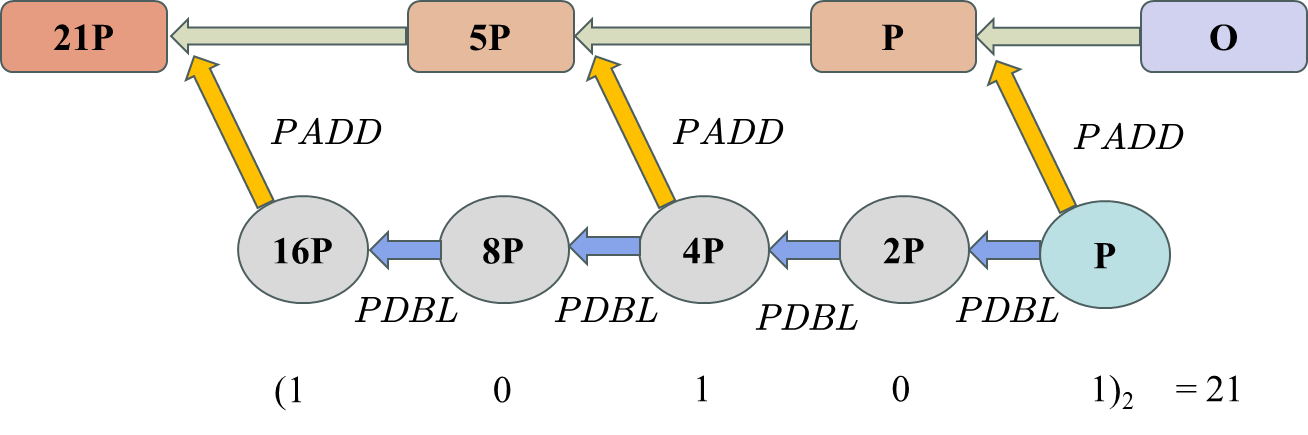
\includegraphics[width=1\linewidth]{image/double-and-add.png}
\caption{The double-and-add algorithm calculates 21P}
\label{fig:double-add}
\end{figure}

Elliptic curve points can be represented using affine coordinates $(x, y)$ or projective coordinates $(X, Y, Z)$. Affine coordinates $(x, y)$ correspond to $(X / Z, Y / Z)$ in projective coordinates. By introducing an auxiliary coordinate $T = XY$, extended projective coordinates $(X, Y, Z, T)$ can be used. Affine coordinates, requiring only two field elements, are efficient for storage but not for point addition due to the expensive modular inversion operation. Projective coordinates avoid this by using $(X, Y, Z)$, and extended projective coordinates $(X, Y, Z, T)$ are even more efficient for point addition.

Most FPGAs implements[] convert points to Edwards curves, which provide fast point addition formulas and more efficient point addition operations. As shown in Eq. \ref{eq:Twisted Edwards}, the Twisted Edwards curve is preferred for fast calculations due to its efficient addition formula. This efficiency arises from the robustness and completeness of the curve, enhancing its performance in cryptographic protocols.
\begin{equation}
a \cdot x^2+y^2=1+d \cdot x^2 \cdot y^2
\label{eq:Twisted Edwards}
\end{equation}

The addition formula of the extended projection coordinates avoids the inefficient modular inversion operation in the Twisted Edwards curve and implements point addition with fewer modular multiplication operations.

Table \ref{tab:field-operations} compares the number of field operations required after applying our transformation. Here, M, S, D, and A represent the number of field multiplications, squares, constant multiplications, and additions or subtractions, respectively.

\begin{table}[htbp]
    \caption{\textbf{Number of field operations for a point addition comparison}}
    \begin{center}
    \begin{tabular}{|c|c|c|c|}
    \hline
    \textbf{Implementation} & \textbf{Curve} & \textbf{Coordinate} & \textbf{Field Operations} \\
    \hline
    RcLboMMSM & Twisted Edwards & Extended & $8M + 1A$ \\
    \hline
    cuZK & Weierstrass & XYZZ & $12M + 2S$ \\
    \hline
    wlc-msm & Weierstrass & XYZZ & $12M + 2S$ \\
    \hline
    DistMSM & Weierstrass & XYZZ & $12M + 2S$ \\
    \hline
    \end{tabular}
    \label{tab:field-operations}
    \end{center}
\end{table}

Compared with previous studies, RcLboMMSM requires only $7M + 8A + 2D$, achieving the least amount of field operations.

\subsection{Multi-scalar Multiplication}

MSM plays a key role in polynomial commitments in zkSNARK. Given N scalars $k_i$ and N elliptic curve points $P_i$, the MSM calculation is defined as shown in Eq. \eqref{eq:MSM}:
\begin{equation}
    \label{eq:MSM}
    Q=\sum_{i=1}^Nk_iP_i
\end{equation}

Multi-scalar multiplication requires a large number of PMUL and PADD operations on elliptic curves.Table \ref{tab:elliptic-curves-bits} lists the number of bits for points and scalars associated with several elliptic curves commonly employed in ZKP.

\begin{table}[htbp]
    \label{tab:elliptic-curves-bits}
    \centering
    \caption{Number of bits for some elliptic curves}
    \begin{tabular}{c|c|c|c|c}
    \toprule
    \textbf{EC} & \textbf{BN254} & \textbf{BLS12-377} & \textbf{BLS12-381} & \textbf{MNT4753} \\
    \midrule
    $k_i$ & 254 bits & 253 bits & 255 bits & 753 bits \\
    $P_i$ & 254 bits & 377 bits & 381 bits & 753 bits \\
    \bottomrule
    \end{tabular}
    \label{tab:elliptic-curves-bits}
\end{table}

Elliptic curve points are typically composed of large finite field elements ranging from 254 to 753 bits. PMUL and PADD operations must be decomposed into modular multiplication and modular addition operations on these large finite fields, which are computationally intensive. Furthermore, the computational cost of multi-scalar multiplication (MSM) is proportional to the size of the point set, which can reach tens of millions. Consequently, MSM is the most time-consuming operation in zkSNARK.

The Pippenger algorithm can be used to reduce the complexity of MSM calculation. Its core idea is to use the distributive law to eliminate PMUL operations. Especially when the MSM scale is very large, the Pippenger algorithm performs best.

\subsection{Pippenger algorithm}
Pippenger provides an asymptotically optimal algorithm for MSM. To this day, the Pippenger algorithm and its variants are still the most advanced and widely used algorithms. To calculate $Q=\sum_{i=1}^N k_i P_i$, the Pippenger algorithm is described as follows(also see a simple example in Figure \ref{fig:pippenger}):

\textbf{1. Task Decomposition}: The Pippenger algorithm selects a window size $c$ and converts each $\lambda$-bit scalar $k_i$ into $\lceil \lambda / c \rceil$ c-bit scalar slices $k_{i,j}$, satisfying Eq \eqref{eq:task-decomposition}:
\begin{equation}
\label{eq:task-decomposition}
\left\{
\begin{aligned}
k_{i,j} &= k_i[j \cdot c : j \cdot c + c - 1] \\
k_i &= \sum_{j=0}^{\lceil \lambda / c \rceil - 1} k_{i,j} 2^{j c}
\end{aligned}
\right.
\end{equation}

Therefore, MSM is decomposed into $\lceil \lambda / c \rceil$ window subtask calculate, satisfying Eq \eqref{eq:task-decomposition-2}:
\begin{equation}
\begin{aligned}
\label{eq:task-decomposition-2}
Q &= \sum_{i=1}^N k_i P_i = \sum_{i=1}^N \sum_{j=0}^{\lambda_c} k_{i,j} 2^{j c} P_i \\
&= \sum_{j=0}^{\lambda_c} 2^{j c} \sum_{i=1}^N (k_{i,j} P_i) \\
&= \sum_{j=0}^{\lambda_c} 2^{j c} Q_j
\end{aligned}
\end{equation}

\textbf{2. Calculate the Window Subtask $Q_j$}: To calculate the subtask result $Q_j$, Pippenger performs the following two stages:
\begin{itemize}
\item \textbf{Bucket Accumulation Stage}: Pippenger introduces a cache point called "bucket". By placing the elliptic curve point $P_i$ with the same scalar value $k_{i,j}$ into a specific bucket with index $k_{i,j}$ ($k_{i,j}$ has $c$ bits, and the bucket corresponding to scalar 0 will not affect the calculation of MSM, so $2^c - 1$ buckets need to be allocated). Add all the points in the same bucket (PADD) to obtain the bucket cumulative value $B_t^{(j)}$, $t \in [1, 2^c - 1]$.
\item \textbf{Bucket Reduction Stage}: The subtask result $Q_j$ is obtained by taking the weighted sum of all buckets according to their bucket index, as shown in Eq \eqref{eq:bucket-reduction}:
\begin{equation}
\label{eq:bucket-reduction}
Q_j = \sum_{i=1}^N k_{i,j} P_i = \sum_{t=1}^{2^c - 1} t B_t
\end{equation}
\end{itemize}

\textbf{3. Window Reduction}: Calculate MSM based on the subtask results. After obtaining the subtask results, the Pippenger algorithm calculates $Q = \sum_{j=0}^{\lambda_c} 2^{j c} Q_j$ to obtain the MSM result.

% \begin{figure}[h]
% \label{fig:pippenger}
% \centering
% 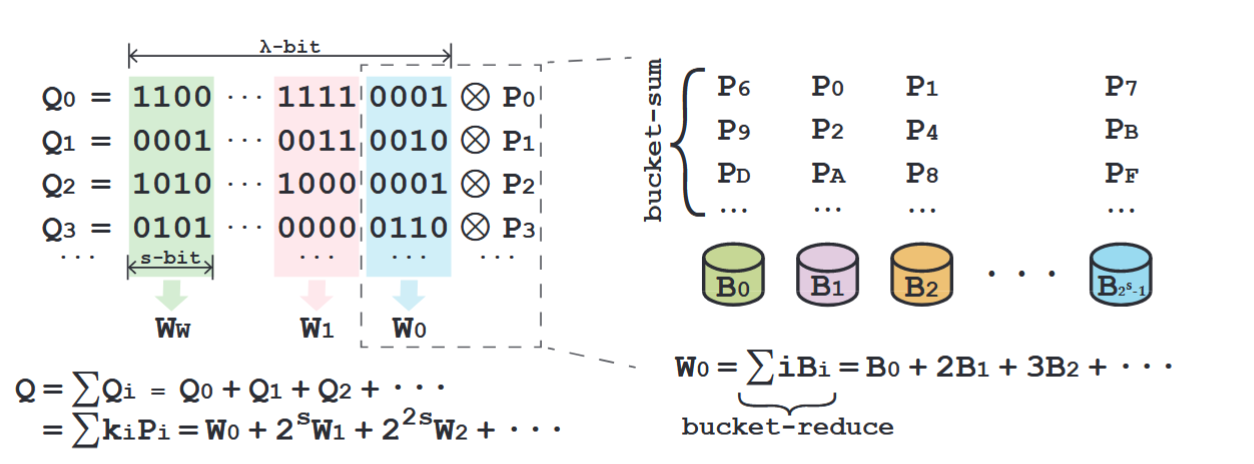
\includegraphics[width=1\linewidth]{image/pippenger.png}
% \caption{llustration of Pippenger algorithm}
% \end{figure}



\begin{figure}[h]
\label{fig:pippenger}
\centering
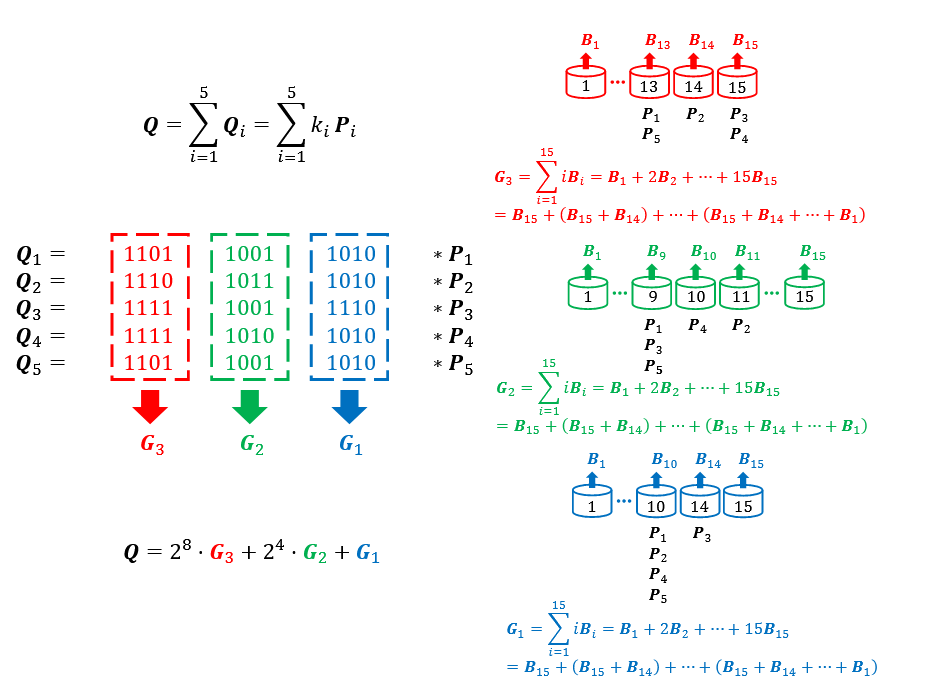
\includegraphics[width=1\linewidth]{image/example-pippenger.png}
\caption{An example of Pippenger algorithm with 5 MSM scale, 12-bit scalars, and window size 4.}
\end{figure}

\subsection{Related work}
\todo{}
ZKP has been successfully applied to electronic voting, verifiable database outsourcing, verifiable machine learning, and verifiable outsourcing. Among ZKP algorithms, zk-SNARK is a practical choice and has been successfully deployed in real-world systems such as ZCash and Pinocchio coin. zk-SNARK provides this dual functionality, ensuring privacy and verifiability for such applications. 

To improve the performance of zk-SNARK proof generation, previous work has focused on implementing high-performance accelerators using GPUs, ASICs, and FPGAs. These accelerators provide efficient solutions for different hardware platforms. PipeZK is an ASIC-based zk-SNARK hardware accelerator that supports multiple curves. It adopts the 4-step algorithm and the Pippenger algorithm in its POLY and MSM accelerators to achieve excellent performance. PipeMSM is an FPGA-based MSM hardware accelerator that introduces innovative PADD design ideas and a high-performance parallel Barrel Aggregation algorithm. CycloneMSM and CycloneNTT are FPGA-based MSM and POLY accelerators developed by the same team. CycloneMSM converts the PADD operation of BLS12-377 into a Twisted Edwards curve, reducing the use of modular multipliers. HARDCAML is also an FPGA-based MSM hardware accelerator that won the 2022 ZPrize championship. It is the best performing FPGA-based MSM accelerator published to date. CuZK and GZKP are high-performance MSM accelerators based on GPUs. CuZK supports parallel execution on multiple GPUs, while GZKP focuses on single GPU performance.

\section{RcLboMMSM Design}
\label{RcLboMMSM Design}
This section introduces the design of the RcLboMMSM, which optimizes MSM for resource-constrained devices. Compared to previous implementations,RcLboMMSM achieves better performance while significantly reducing resource usage, supporting larger-scale MSM computations. Furthermore, the framework supports not only single GPU but also multi-GPU environments. It dynamically allocates tasks based on different hardware resources to ensure load balancing, thereby efficiently processing large-scale MSM tasks.
\subsection{RcLboMMSM Design for Single GPU}
This section introduces the design of the RcLboMMSM framework for single GPU, especially consumer-grade GPUs, which optimizes MSM for resource-constrained devices. The details are described as follows, as shown in Algorithm \ref{alg:rclbomsm-single-gpu}.

\begin{algorithm}
    \caption{RcLboMMSM Single GPU Pseudocode Algorithm}
    \label{alg:rclbomsm-single-gpu}
    \begin{algorithmic}[1]
    \REQUIRE Scalar vector $\overrightarrow{k_N} = [k_1, k_2, \ldots, k_N]$, each $k_i$ is a $\lambda$-bit scalar; point vector $\overrightarrow{P_N} = [\mathbf{P}_1, \mathbf{P}_2, \ldots, \mathbf{P}_N]$
    \ENSURE Compute $\mathbf{Q} = \sum_{i=1}^{N} k_i \mathbf{P}_i$
    \STATE Transfer $\overrightarrow{P}_N$ to GPU and convert to Twisted Edwards extend coordinates system
    \STATE Precompute points, store them in GPU memory, and allocate the necessary GPU resources.
    \STATE Select optimal window size $c$ and compression coefficient M based on the curve type, input size, and GPU resources
    \STATE Convert scalars $\overrightarrow{k_n}$ to signed form 
    \FOR{each window $j = 0$ to $\lceil \lambda / c \rceil - 1$}
        \STATE Sort scalar slices $k_{i,j}$ and corresponding points $\mathbf{P}_i$ by $k_{i,j}$
        \STATE Accumulate points into buckets using shared memory 
        \STATE Perform bucket reduction to compute local sums 
    \ENDFOR
    \STATE Perform inter-window reduction on GPU to obtain partial results
    \STATE Transfer partial results to CPU and complete final reduction to compute $\mathbf{Q}$
    \RETURN $\mathbf{Q}$
    \end{algorithmic}
\end{algorithm}
\subsubsection{\textbf{Optimal Window Size Selection}}

The window size \( c \) is a critical parameter that affects both the parallelism of the MSM module and the distribution of bucket workloads, thereby significantly influencing overall computational efficiency. Generally, larger window sizes decrease the total computational cost of the Pippenger algorithm in MSM. However, increasing \( c \) also markedly raises the number of bucket reduction tasks, introducing new performance challenges.

Furthermore, various elliptic curve properties, input point set distributions, and device resources may respond differently to varying window sizes, and their impact on the total computation time cannot be overlooked. Therefore, thoughtfully selecting the window size is essential to optimize performance, taking into account specific curve characteristics, input point set properties, and available hardware resources.

To determine the optimal window size \( c \), we employ an offline search strategy. Initially, we conduct preliminary experiments to gather performance data for various window sizes across different data scales and GPU devices. By executing benchmark MSM tasks with varying window sizes \( c \) on the GPU, we record performance metrics such as execution time and memory usage, thereby creating a comprehensive performance map. Recognizing that in practical ZKP applications, GPUs are not exclusively dedicated to MSM acceleration, the actual memory constraints may be lower than the GPU's total device memory. Leveraging this performance map, we select the window size that offers the best trade-off between computational efficiency and memory usage, ensuring it adheres to the memory limitations of the target GPU. The detailed search algorithm is outlined in Algorithm \ref{alg:optimal-window-size}.
\begin{algorithm}
    \caption{Optimal Window Size Selection}
    \label{alg:optimal-window-size}
    \begin{algorithmic}[1]
    \REQUIRE Data scale, GPU specifications, memory constraints, experimental map
    \ENSURE Optimal window size \( c^* \)
    \STATE Initialize a list of candidate window sizes \( C = \{c_1, c_2, \ldots, c_n\} \)
    \FOR{each \( c \in C \)}
        \IF{Memory usage with window size \( c \) exceeds constraints}
            \STATE Skip window size \( c \)
        \ENDIF
    \ENDFOR
    \IF{No window sizes satisfy memory constraints}
        \STATE \textbf{Return} an error or default to the smallest window size
    \ELSE
        \STATE Select the window size \( c^* \) from the experimental map that offers the best trade-off between performance and resource utilization
    \ENDIF
    \RETURN \( c^* \)
    \end{algorithmic}
\end{algorithm}

\subsubsection{\textbf{Elastic Precomputation}}
The precomputation method reduces running time by generating a series of elliptic curve (EC) points in advance and treating them as additional base points in the MSM. However, this approach increases the number of points by several times compared to the original base points. Consequently, storing these points in GPU memory during runtime results in significant storage overhead, posing a challenge for large-scale MSM computations.

To better balance time and space overhead, this paper adopts the elastic precomputation scheme. Elastic precomputation offers a trade-off between the runtime of the Pippenger algorithm and the additional GPU storage space required. This flexibility allows for an adjustable amount of preprocessing based on specific needs, optimizing performance while accommodating various storage constraints, especially in resource-constrained environments.

Specifically, this paper sets the precomputation compression coefficient \( M \) as a control parameter to manage the time and space trade-off, thereby adjusting the data that needs to be precomputed. The precomputed points to be calculated are shown in Eq. \eqref{eq:precomputation}.

\begin{equation}
\label{eq:precomputation}
    2^{Mc} P_i, \, 2^{(2M) \cdot c} P_i, \, \ldots, \, 2^{\left(\left\lceil \frac{\lceil \lambda / c \rceil}{M} \right\rceil - 1\right) \cdot Mc} P_i
\end{equation}

By setting the compression coefficient $M$, the original number of windows can be reduced to $M$. However, this paper does not utilize this technique to reduce bucket space, as we aim to prevent different threads from accessing the same bucket and causing conflicts. In the bucket accumulation phase, we continue to use the original subtask division and add the corresponding flattened weighted precomputed points to the window buckets. After completing bucket accumulation, we allocate threads to perform cross-window bucket reduction, reducing the number of windows to $M$, and then complete the intra-window bucket reduction and CPU-side window reduction on these $M$ windows.


\subsubsection{\textbf{Scalar conversion and Twisted Edwards Coordinates}}
\textbf{Scalar conversion: } In the Pippenger algorithm, re-encoding the scalar into a signed binary form in advance can effectively reduce the number of buckets by half, reducing memory overhead while also reducing the time overhead of bucket reduction. 

Specifically, this paper converts the scalar $k_i$ from an unsigned c-bit binary representation to a signed representation of each scalar slice in the range of $\left[-2^{c-1}, 2^{c-1}\right]$, as shown in Eq. \eqref{eq:sclar-transformation}. The specific details of the conversion algorithm are shown in Algorithm \ref{alg:scalar-transformation}.

\begin{equation}
\label{eq:sclar-transformation}
k_i=\sum_{j=0}^{\lambda} k_{i, j}=\sum_{j=0}^{\lambda} \bar{k}_{i, j} \cdot(-1)^{s_{i, j}}
\end{equation}

\begin{algorithm}
\label{alg:scalar-transformation}
\caption{Scalar Transformation Algorithm}
\begin{algorithmic}[1] % [1] 表示为每行添加行号
\REQUIRE Bit-length $\lambda$, window size $c$, $N$ scalars $\{k_i\}_{i \in [N]}$
\ENSURE Tuple $\{\widetilde{k}_{i,j}, s_{i,j}\}$

\STATE $s_{i,-1} \gets 0$, $t \gets 0$
\FOR{$j = 0$ \textbf{to} $\lceil \lambda / c \rceil$}
    \STATE $k_{i,j} \gets k_i[jc : jc + c - 1]$
    \STATE $t \gets k_{i,j} + s_{i,j-1}$
    \STATE $s_{i,j} \gets \textbf{if } t > 2^{c-1} \textbf{ then } 1 \textbf{ else } 0$
    \STATE $\widetilde{k}_{i,j} \gets \textbf{if } t > 2^{c-1} \textbf{ then } t - 2^c \textbf{ else } t$
\ENDFOR

\end{algorithmic}
\end{algorithm}

\textbf{Twisted Edwards Coordinates:} For specific ZKP applications and curves, curve transformations are precomputed; the primary task is point transformation. Algorithm \ref{alg:twisted_edwards_transformation} outlines the conversion to the Twisted Edwards curve. Initially, points are transformed from the Weierstrass form to the Montgomery curve as shown in Eq. \eqref{eq:montgomery} ($A$ and $B$ are curve parameters):

\begin{equation}
\label{eq:montgomery}
B y^2 = x^3 + A x^2 + x
\end{equation}

Subsequently, the Montgomery curve is converted to the Twisted Edwards curve. However, not all points can be mapped this way. Points where \( x_{\text{mont}} = -1 \) or \( y_{\text{mont}} = 0 \) on the Twisted Edwards curve are invalid. These points are filtered out on the CPU, and their contributions to the MSM result are computed by the CPU without conversion.

\begin{algorithm}[H]
\caption{Transformation to Twisted Edwards Coordinates}
\label{alg:twisted_edwards_transformation}
\begin{algorithmic}[1]
\REQUIRE Elliptic curve parameters \( a, b \) in Weierstrass form.
\ENSURE Transformed points on the Twisted Edwards curve.

\STATE Compute \( s = (\sqrt{3 a^2 + a})^{-1} \).
\STATE Find root \( \alpha \) of \( x^3 + a x + b = 0 \).
\STATE Set \( A = 3 \alpha s \) and \( B = s \).
\STATE Compute Twisted Edwards parameters:
\begin{align*}
a' &= \frac{A + 2}{B} \\
d &= \frac{A - 2}{B}
\end{align*}
\FOR{each point \( (x_{\text{weierstrass}}, y_{\text{weierstrass}}) \)}
    \STATE Compute Montgomery coordinates:
    \begin{align*}
    x_{\text{mont}} &= s (x_{\text{weierstrass}} - a) \\
    y_{\text{mont}} &= s \cdot y_{\text{weierstrass}}
    \end{align*}
    \STATE Compute Twisted Edwards coordinates:
    \begin{align*}
    x_{\text{twist}} &= \frac{x_{\text{mont}}}{y_{\text{mont}}} \\
    y_{\text{twist}} &= \frac{x_{\text{mont}} - 1}{x_{\text{mont}} + 1}
    \end{align*}
    \IF{ \( x_{\text{mont}} = -1 \) or \( y_{\text{mont}} = 0 \) }
        \STATE \textbf{Filter out} the point and handle MSM contribution on the CPU.
    \ENDIF
    \STATE \textbf{Store} \( (x_{\text{twist}}, y_{\text{twist}}) \)
\ENDFOR
\end{algorithmic}
\end{algorithm}

\subsubsection{\textbf{Reducing Register Pressure in PADD Operations}}
Optimizing the Point Addition (PADD) operation for large integers heavily relies on managing register pressure—the demand for available registers by concurrent live variables—which directly impacts the kernel's occupancy rate. In PADD operations, each multiplication involves complex large integer modular arithmetic, necessitating numerous computations, memory accesses, and synchronization steps. To mitigate register pressure, RcLboMMSM, similar to DistMSM, rearranges PADD operations in extended coordinates to minimize the peak number of active large integers at any given time.

As illustrated in Figure \ref{fig:padd-register}, this paper analyzed the PADD operation on the Twisted Edwards curve and proposed an optimal execution order accordingly.

\begin{figure}[h]
    \centering
    \label{fig:padd-register}
    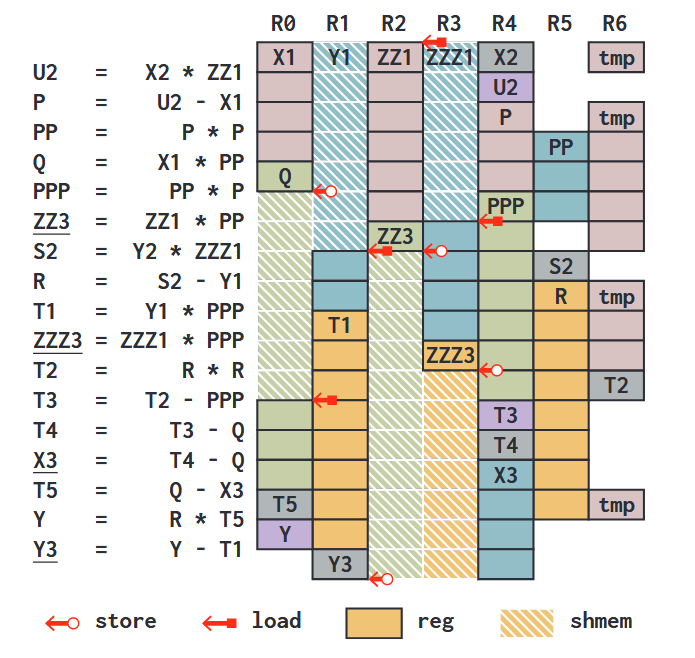
\includegraphics[width=1\linewidth]{image/padd_register.png}
    \caption{Optimal Execution Order of PADD Operation}
\end{figure}

\subsubsection{\textbf{Bucket accumulation load balancing optimized for applications}}
Zero-knowledge proof applications frequently encounter uneven scalar data distributions. In real-world workloads, scalars are highly sparse due to extensive boundary checks and range constraints during system setup, as illustrated in Figure \todo{}. This prevalence of numerous 0s and 1s results in significant load imbalances in some existing systems.

This paper adopts the load balancing scheme from wlc-msm, which addresses conflict issues by pre-allocating non-conflicting point buffers, caching points within these buffers, and utilizing binary search to assign points to their corresponding buckets.

Specifically, during the bucket accumulation phase, points are written to a pre-allocated non-conflicting static buffer for each thread instead of directly into the buckets. For each of the $\lceil\lambda/ c \rceil$ subtasks, a static buffer is allocated, and the starting offset for each thread's writes to the buffer is determined by the provided Eq. \ref{eq:buffer-offset}.
\
\begin{equation}
    \label{eq:buffer-offset}
    \left\{\begin{aligned} {{{}}} & {{} {{} {{} o f f s e t_{t i d}=t i d+\operatorname* {m i n} \left\{a_{i} \right\}_{i \in[ s, c )}}}} \\ {{{}}} & {{} {{} {{} [ s, e )=\left[ \left[ n / N \right] \cdot t i d, \left[ n / N \right] \cdot( t i d+1 ) \right)}}} \\ \end{aligned} \right. 
\end{equation}

Where $a_{i}$ is the $i$th scalar in the sorted subtask. The maximum buffer offset is $N+2^{c-1}$, so the total size of the static buffer that needs to be allocated is $\lceil\lambda/ c \rceil\cdot( N+2^{c-1} )$. In addition, in order to write the points stored in the buffer to the corresponding buckets later, three auxiliary arrays need to be allocated: buffer\_offset is used to store the starting position of the thread writing to the buffer; buffer\_index is used to store the bucket offset corresponding to the write point; buffer\_use is used to store the buffer size actually used by the thread. The buffer needs to store elliptic curve points. The three auxiliary arrays only need to store numbers. They take up very little space, namely: 
\begin{equation} \left\{ 
    \begin{aligned} 
        \ & \lceil \lambda / c \rceil \cdot N \\ \ & \lceil \lambda / c \rceil \cdot (N + 2^{c-1}) \\ \ & \lceil \lambda / c \rceil \cdot N 
    \end{aligned} \right. 
\end{equation}

Specifically, in the bucket accumulation phase, we need to complete three stages of operations:
\begin{itemize}
    \item \textbf{Sort the preprocessed sub-scalars and point indices:} For each subtask, in the bucket accumulation phase, the tuple $\{\widetilde{k}_{i,j}, s_{i,j}\}$ needs to be sorted based on the key $\widetilde{k}_{i,j}$. This paper uses the radix sort algorithm provided by the CUDA CUB library.
    \item \textbf{Write to the static buffer:} Accumulate points into the buffer. Before accumulating points into the buffer, the subtask needs to find the precomputed points that need to be added to the bucket instead of the original points. It needs to find the corresponding precomputed points in the precomputed point set based on the subtask number. On this basis, this paper uses the load balancing scheme proposed by wlc-msm, as shown in Algorithm \ref{alg:shared-memory-accumulation}. Similar to wlc-msm, this paper uses shared memory to accelerate the read and write of precomputed points, accumulates points into the subtask static buffer, and records the corresponding values in the three auxiliary arrays buffer\_offset, buffer\_index, and buffer\_used to facilitate the next step of accumulating points into the corresponding buckets.
    \item \textbf{Accumulate buffer points into buckets:} Since the subtask has completed the sorting of scalars and point indices, the bucket offsets corresponding to the points stored in the buffer are also sorted in ascending order. Binary search can be used to complete the accumulation task. For each subtask, this paper allocates $2^c-1$ threads, where the thread with index tid is used to search for all buffer points corresponding to bucket ($tid+1$) B and accumulate the buffer points back to the unique bucket (bucket 0 does not contribute to the MSM calculation).
\end{itemize}

\begin{algorithm}
    \caption{Using Shared Memory to Accumulate Points to Buffer}
    \label{alg:shared-memory-accumulation}
    \begin{algorithmic}[1]
    \REQUIRE Sorted tuple pairs $\{(a_i, p_i)\}_{i \in [N]}$, precomputed point set $\{P_i\}_{i \in [N]}$
    \ENSURE Static buffer \texttt{buffer}, three auxiliary arrays \texttt{buffer\_offset}, \texttt{buffer\_index}, \texttt{buffer\_used}
    
    \STATE Obtain boundaries $[s, e)$
    \STATE $\text{pre\_bucket\_idx} = 0xffff$ \COMMENT{Non-existent bucket index}
    \STATE $\text{buffer\_offset}[\text{tid}] = \text{offset} = \text{tid} + (a_s >> 1)$
    \STATE $\text{num} = 0$
    \STATE $\text{smem}[2 \cdot \text{tid\_inner} + 1] = O$ \COMMENT{$\text{tid\_inner}$ and $O$ are thread block index and elliptic curve point at infinity}
    \FOR{$i = s$ to $e - 1$}
        \STATE $\text{cur\_bucket\_idx} = a_s >> 1$
        \IF{$\text{cur\_bucket\_idx} \neq \text{pre\_bucket\_idx}$ and $i \neq s$}
            \STATE $\text{buffer}[\text{offset} + \text{num}] = \text{smem}[2 \cdot \text{tid\_inner} + 1]$
            \STATE $\text{buffer\_index}[\text{offset} + \text{num}] = \text{pre\_bucket\_idx}$
            \STATE $\text{smem}[2 \cdot \text{tid\_inner} + 1] = O$
            \STATE $\text{num} = \text{num} + 1$
        \ENDIF
        \STATE $\text{pre\_bucket\_idx} = \text{cur\_bucket\_idx}$
        \STATE $\text{smem}[2 \cdot \text{tid\_inner}] = P[p_i]$ \COMMENT{Find the precomputed point}
        \IF{$(a_i \& 1)$}
            \STATE $\text{smem}[2 \cdot \text{tid\_inner}] = -\text{smem}[2 \cdot \text{tid\_inner}]$
        \ENDIF
        \STATE $\text{smem}[2 \cdot \text{tid\_inner} + 1] = \text{PADD}(\text{smem}[2 \cdot \text{tid\_inner} + 1], \text{smem}[2 \cdot \text{tid\_inner}])$
    \ENDFOR
    
    \STATE $\text{buffer}[\text{offset} + \text{num}] = \text{smem}[2 \cdot \text{tid\_inner} + 1]$
    \STATE $\text{buffer\_index}[\text{offset} + \text{num}] = \text{pre\_bucket\_idx}$
    \STATE $\text{buffer\_used}[\text{tid}] = \text{num} + 1$
\end{algorithmic}
\end{algorithm}


\subsubsection{\textbf{Bucket aggregation optimization}}
This paper refines the bucket reduction operation of the original Pippenger algorithm into cross-window and intra-window bucket reductions. During preprocessing and bucket accumulation stages, bucket weights are flattened, meaning that every M windows, the corresponding bucket weights are the same. For example, the 0th window can be directly added to the Mth window, compressing the original window into M. In M windows, threads perform bucket reduction on buckets with the same weights in the remaining windows. This way, more points are added to the same bucket, maximizing the advantages of the Pippenger algorithm. Next, the bucket reduction within the M windows is completed. The MSM calculation is particularly bottlenecked by the bucket reduction stage of the Pippenger algorithm, which is essentially a sequential workload, as shown in Figure \ref{fig:bucket_reduction}. To parallelize this stage, we propose Algorithm \ref{alg:cross-intra-bucket-reduction}.

\begin{algorithm}
    \caption{Cross-Window and Intra-Window Bucket Reduction}
    \label{alg:cross-intra-bucket-reduction}
    \begin{algorithmic}[1]
    \REQUIRE Bucket vector $\vec{B}_{2^c - 1} = [B_1, B_2, \ldots, B_{2^c - 1}]$, window size $c$, compression coefficient $M$, thread count $n$, global memory $sos$
    \ENSURE MSM result $Q$
    \STATE Initialize $Q = 0$
    \FOR{each window group $g = 0$ to $\lceil \lambda / (Mc) \rceil - 1$}
        \STATE Initialize $Q_g = 0$
        \FOR{each window $j = 0$ to $M - 1$}
            \STATE Initialize $Q_{g,j} = 0$
            \FOR{each bucket $t = 1$ to $2^c - 1$}
                \STATE $Q_{g,j} = Q_{g,j} + t \cdot B_{g \cdot M + j, t}$
            \ENDFOR
        \ENDFOR
        \STATE $Q_g = \sum_{j=0}^{M-1} 2^{jc} \cdot Q_{g,j}$
    \ENDFOR
    \STATE $Q = \sum_{g=0}^{\lceil \lambda / (Mc) \rceil - 1} 2^{gMc} \cdot Q_g$
    \STATE Obtain thread processing boundaries $[s, e]$ \quad // Each thread processes $(2^c - 1 + n - 1) / n$ parts
    \STATE $sos\_tmp = 0$; $st\_tmp = 0$; $tmp = 0$
    \FOR{$i = e - 1$ \TO $s$}
        \STATE $st\_tmp = PADD(st\_tmp, B[i])$
        \STATE $sos\_tmp = PADD(sos\_tmp, st\_tmp)$
        \STATE $tmp = mul(tid \cdot step\_len, st\_tmp)$
        \STATE $sos[tid] = PADD(sos\_tmp, tmp)$
    \ENDFOR
    \STATE \_\_syncthreads()
    \STATE $Q = reduce\_sum(sos, n)$ \quad // Parallel sum of $sos$
    \RETURN $Q$
    \end{algorithmic}
\end{algorithm}

\begin{figure}[h]
    \centering
    \label{fig:bucket_reduction}
    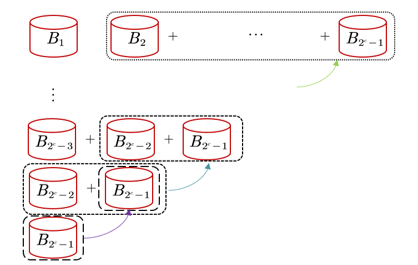
\includegraphics[width=1\linewidth]{image/bucket_reduction.png}
    \caption{Serial Execution of Bucket Reduction}
\end{figure}


\subsection{RcLboMMSM Design for Multi-GPU Systems}

While previous research has primarily focused on optimizing single-device performance or introducing new protocols for distributed systems, these approaches often exhibit limitations in practical applications and face challenges in achieving universal scalability.

To overcome these limitations, we propose a hierarchical partitioning framework within our RcLboMMSM design, which extends to support multi-GPU systems. This framework divides the MSM task into multiple layers based on data scale and hardware characteristics. By employing an optimal sub-window search strategy, we efficiently allocate tasks within the computational resources of one or multiple GPUs, achieving better load balancing and performance. The RcLboMMSM system dynamically allocates tasks across GPUs based on data size and hardware resources, ensuring efficient utilization of all available computational resources. The hierarchical design and its extension to multi-GPU systems are illustrated in Figures \ref{fig:RcLboMMSM_multi_gpu_framework}

\begin{figure}[h]
\centering
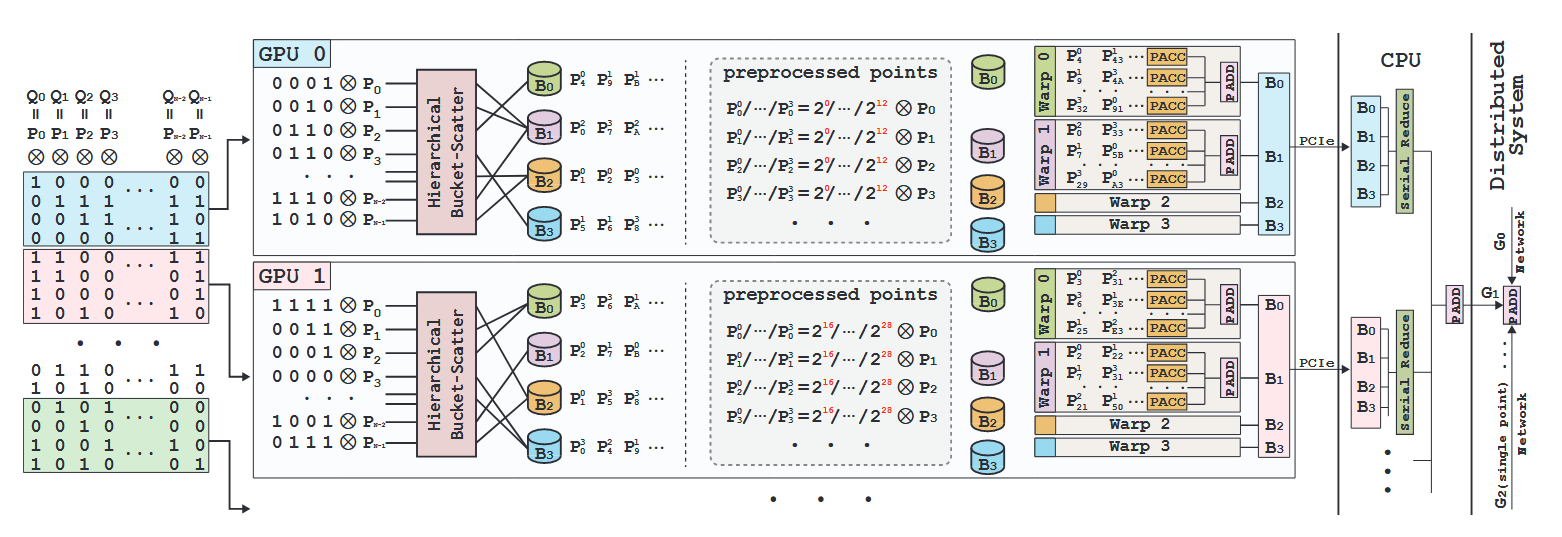
\includegraphics[width=1\linewidth]{image/framework.png}
\caption{Hierarchical Partitioning Framework in RcLboMMSM Design}
\label{fig:RcLboMMSM_multi_gpu_framework}
\end{figure}


\section{Evaluation}
\label{sec:Evaluation}

Our evaluation comprises three parts: assessing the overall performance of MSM operations on a single GPU, evaluating performance on multi-GPU systems, and providing a detailed analysis of the proposed optimizations. The experiments were conducted on three different GPU servers rented from the AutoDL platform, namely RTX 4090, V100, and A40. Table \ref{tab:hardware-config} presents the hardware specifications, including the CPU configuration. Since the MSM implementation primarily runs on the GPU, CPU performance mainly affects the scalar data transfer time between the host and device. To ensure a fair comparison, all benchmark implementations were executed on the same test platform. Although our framework supports load balancing across different graphics cards in a multi-GPU environment, due to limitations in our experimental setup, we conducted tests using multiple identical RTX 4090 GPUs.

\begin{table}[htbp]
    \caption{\textbf{Hardware Configuration of Testing Environments}} % Title of the table
    \centering
    \begin{tabular}{|c|c|c|c|}
    \hline
    \textbf{Environment} & \textbf{RTX 4090} & \textbf{V100} & \textbf{A40} \\
    \hline
    SM Count & 128 & 80 & 128  \\
    \hline
    Memory & 24GB & 32GB & 48GB  \\
    \hline
    OS & Ubuntu 20.04 & Ubuntu 20.04 & Ubuntu 20.04 \\
    \hline
    CUDA Version & 11.8 & 11.8 & 11.8 \\
    \hline
    \end{tabular}
    \label{tab:hardware-config} % Label for referencing
\end{table}

We utilize the Zprize-provided testing framework, where the point set for evaluating multi-scalar multiplication (MSM) is randomly generated. There are two types of scalars: random scalars sampled from the scalar domain and clustered scalars as proposed by cuZK. In practical applications, scalars are not uniformly random; thus, evaluating MSM performance using only random scalars and point sets is insufficient. Therefore, we adopt a second evaluation standard using clustered scalars, limiting scalars to 32 distinct values to reflect more realistic distributions.

We compare our implementation against several leading GPU-based MSM implementations (Table \ref{tab:baseline-gpu-implementations}).
\begin{table}[htbp]
    \caption{\textbf{Baseline GPU Implementations Used for Evaluation}} % Title of the table
    \begin{center}
    \begin{tabular}{|c|c|c|}
    \hline
    \textbf{Baseline} & \textbf{Supported Elliptic Curves} & \textbf{GPU Support} \\
    \hline
    wlc-msm & BLS12-377, BLS12-381 & Single GPU \\
    \hline
    Yrrid & BLS12-377 & Single GPU \\
    \hline
    GZKP & ALT-BN128, BLS12-381, MNT4753 & Single GPU \\
    \hline
    Bellperson & BLS12-381 & Multi GPU \\
    \hline
    Sppark & BLS12-377, BLS12-381, BN254 & Multi GPU \\
    \hline
    cuZK & BLS12-377, BLS12-381, MNT4753 & Multi GPU \\
    \hline
    \end{tabular}
    \label{tab:baseline-gpu-implementations} % Add a label for referencing
    \end{center}
\end{table}


\subsection{Overall Performance for sigle GPU}
\todo{}

\subsection{Overall Performance for sigle GPU}
\todo{}

\subsection{Breakdown Analysis}
\todo{}
\section{Conclusion}
\todo{}
\section*{Acknowledgment}

The preferred spelling of the word ``acknowledgment'' in America is without 
an ``e'' after the ``g''. Avoid the stilted expression ``one of us (R. B. 
G.) thanks $\ldots$''. Instead, try ``R. B. G. thanks$\ldots$''. Put sponsor 
acknowledgments in the unnumbered footnote on the first page.

\section*{References}

Please number citations consecutively within brackets \cite{b1}. The 
sentence punctuation follows the bracket \cite{b2}. Refer simply to the reference 
number, as in \cite{b3}---do not use ``Ref. \cite{b3}'' or ``reference \cite{b3}'' except at 
the beginning of a sentence: ``Reference \cite{b3} was the first $\ldots$''

Number footnotes separately in superscripts. Place the actual footnote at 
the bottom of the column in which it was cited. Do not put footnotes in the 
abstract or reference list. Use letters for table footnotes.

Unless there are six authors or more give all authors' names; do not use 
``et al.''. Papers that have not been published, even if they have been 
submitted for publication, should be cited as ``unpublished'' \cite{b4}. Papers 
that have been accepted for publication should be cited as ``in press'' \cite{b5}. 
Capitalize only the first word in a paper title, except for proper nouns and 
element symbols.

For papers published in translation journals, please give the English 
citation first, followed by the original foreign-language citation \cite{b6}.

\begin{thebibliography}{00}
\bibitem{b1} G. Eason, B. Noble, and I. N. Sneddon, ``On certain integrals of Lipschitz-Hankel type involving products of Bessel functions,'' Phil. Trans. Roy. Soc. London, vol. A247, pp. 529--551, April 1955.
\bibitem{b2} J. Clerk Maxwell, A Treatise on Electricity and Magnetism, 3rd ed., vol. 2. Oxford: Clarendon, 1892, pp.68--73.
\bibitem{b3} I. S. Jacobs and C. P. Bean, ``Fine particles, thin films and exchange anisotropy,'' in Magnetism, vol. III, G. T. Rado and H. Suhl, Eds. New York: Academic, 1963, pp. 271--350.
\bibitem{b4} K. Elissa, ``Title of paper if known,'' unpublished.
\bibitem{b5} R. Nicole, ``Title of paper with only first word capitalized,'' J. Name Stand. Abbrev., in press.
\bibitem{b6} Y. Yorozu, M. Hirano, K. Oka, and Y. Tagawa, ``Electron spectroscopy studies on magneto-optical media and plastic substrate interface,'' IEEE Transl. J. Magn. Japan, vol. 2, pp. 740--741, August 1987 [Digests 9th Annual Conf. Magnetics Japan, p. 301, 1982].
\bibitem{b7} M. Young, The Technical Writer's Handbook. Mill Valley, CA: University Science, 1989.
\end{thebibliography}
\vspace{12pt}

\end{document}
